%\documentclass[12pt]{article}
%\usepackage{graphicx}
%\usepackage{times}
%\usepackage{calrsfs}
%\usepackage{mathrsfs}
%\usepackage{cite}
%\usepackage{rotating}
%\usepackage[T1]{fontenc}


%\setlength{\parindent}{0.0cm}
%\setlength{\parskip}{0.5cm}
%\setlength{\textheight}{8.8in}
%\setlength{\textwidth}{6.5in}
%\setlength{\topmargin}{0pt}
%\setlength{\oddsidemargin}{0pt}
%\setlength{\evensidemargin}{0pt}
%\setlength{\marginparwidth}{44pt}
%\renewcommand{\baselinestretch}{1.2}


%\newcommand{\eg}{{\it e.g.~}}
%\newcommand{\ie}{{\it i.e.~}}

%\newcommand{\NAMDCONF}[4]{
%  {\bf \tt #1 } $<$ #2 $>$ \\
%  {\bf Acceptable Values: } #3 \\
%  {\bf Description: } #4
%}

%\newcommand{\NAMDCONFWDEF}[5]{
%  {\bf \tt #1 } $<$ #2 $>$ \\
%  {\bf Acceptable Values: } #3 \\
%  {\bf Default Value: } #4 \\
%  {\bf Description: } #5
%}



%\begin{document}


%\addtolength{\baselineskip}{0.2\baselineskip}


%\setlength{\abovedisplayshortskip}{-0.6cm}
%\setlength{\abovedisplayskip}{-0.6cm}
%\setlength{\belowdisplayshortskip}{0.5cm}
%\setlength{\belowdisplayskip}{0.5cm}


%\renewcommand{\rightmark}{\footnotesize{\it Alchemical free energy
%                                            calculations in NAMD}}



%%%%%%%%%%%%%%%%%%%%%%%%%%%%%%%%%%%%%%%%%%%%%%%%%%%%%%%%%%%%%%%%%%%%%%%%%%%%%%%%%
%%% TEXT
%%%%%%%%%%%%%%%%%%%%%%%%%%%%%%%%%%%%%%%%%%%%%%%%%%%%%%%%%%%%%%%%%%%%%%%%%%%%%%%%%

%\title{User guide to the alchemical free energy
%       calculations in NAMD}





%\maketitle


%\thispagestyle{empty}


%\newpage


%\pagestyle{headings}

\section{Alchemical Free Energy Methods\footnote[1]{The features described in this section were contributed by Surjit B. Dixit, J\'{e}r\^{o}me H\'{e}nin, Christophe Chipot (Nancy Universit{\'e}, Universit{\'e} Henri Poincar{\'e}, France), Floris Buelens (Institute of Structural and Molecular Biology, University of London, United Kingdom), and Christopher Harrison (University of Illinois, USA).}}
\label{section:alchemy}

Alchemical free energy calculations model the physically impossible but
computationally realizable process of gradually mutating a subset of atoms of a
system from one state to another, through a series of intermediate steps. Two
alternative methods for alchemical calculation of free energies from molecular
dynamics simulation are available in NAMD: Free energy perturbation (FEP) and
thermodynamic integration (TI).
%CBH INSERT FOOTNOTE HERE  -- Surjit B. Dixit, J\'{e}r\^{o}me H\'{e}nin and Christophe Chipot (Nancy Universit{\'e}, Universit{\'e} Henri Poincar{\'e}, France), and Floris Buelens (Institute of Structural and Molecular Biology, Birkbeck / UCL, University of London, United Kingdom), etc, etc.



\subsection{Theoretical Background}

Free energy differences can be obtained through four different routes: (i)
probability densities, (ii) free energy perturbation, (iii) thermodynamic
integration, or (iv) nonequilibrium work approaches~\cite{Chipot2007}.  Within
NAMD, alchemical transformations are modeled following the second and the third
routes, both of which rely upon the use of a general extent parameter often
referred to as the coupling
parameter~\cite{Beveridge1989,Mark1998,King1993,Kirkwood1935} for the
description of chemical changes in the molecular systems between the reference
and the target states.


\subsubsection{The dual--topology paradigm}


In a typical alchemical transformation setup involving the alteration of one
chemical species into an alternate one in the course of the simulation, the
atoms in the molecular topology can be classified into three groups, (i) a
group of atoms that do not change during the simulation --- \eg the
environment, (ii) the atoms describing the reference state, $a$, of the
system, and (iii) the atoms that correspond to the target state, $b$, at the
end of the alchemical transformation. The atoms representative of state $a$
should \emph{never} interact with those of state $b$ throughout the MD
simulation. Such a setup, in which atoms of both the initial and the final
states of the system are present in the molecular topology file --- \ie the
{\tt psf} file --- is characteristic of the so--called ``dual topology''
paradigm~\cite{Gao1989,Pearlman1994a,Axelsen1998}. The hybrid Hamiltonian
of the system is a function of the general extent parameter, $\lambda$,
which connects smoothly state $a$ to state $b$. In the simplest case, such a
connection may be achieved by linear combination of the corresponding Hamiltonians:

\begin{equation}
{\cal H}({\bf x}, {\bf p}_x; \lambda)
                  = {\cal H}_0({\bf x}, {\bf p}_x)
                  + \lambda {\cal H}_b({\bf x}, {\bf p}_x)
                  + (1-\lambda) {\cal H}_a({\bf x}, {\bf p}_x)
\label{linear}
\end{equation}


\noindent where ${\cal H}_a({\bf x}, {\bf p}_x)$ describes the interaction of
the group of atoms representative of the reference state, $a$, with the rest of
the system. ${\cal H}_b({\bf x}, {\bf p}_x)$ characterizes the interaction of
the target topology, $b$, with the rest of the system. ${\cal H}_0({\bf x},
{\bf p}_x)$ is the Hamiltonian describing those atoms that do not undergo any
transformation during the MD simulation.


For instance, in the point mutation of an alanine side chain into that of
glycine, by means of a free energy calculation --- either free energy
perturbation or thermodynamic integration, the topology of both the methyl
group of alanine and the hydrogen borne by the C$_\alpha$ in glycine co--exist
throughout the simulation (see Figure~\ref{fig:dual_top}), yet without actually
seeing each other.


\begin{figure}[ht]
  \center{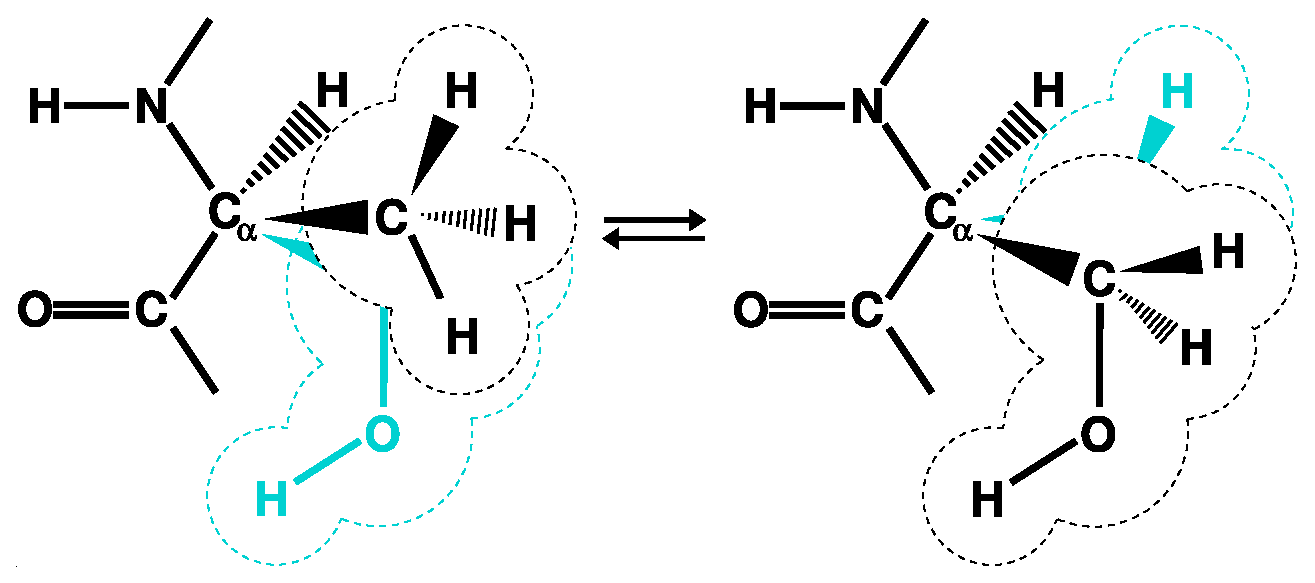
\includegraphics[width=12.5cm]{figures/dual_top}}
  \caption{Dual topology description for an alchemical simulation.
           Case example of the mutation of alanine into serine.
           The lighter color denotes the non--interacting, alternate
           state.
           \label{fig:dual_top}}
\end{figure}


The energy and forces are defined as a function of $\lambda$, in such a fashion
that the interaction of the methyl group of alanine with the rest of the
protein is effective at the beginning of the simulation, \ie  $\lambda$ = 0,
while the glycine C$_\alpha$ hydrogen atom does not interact with the rest of
the protein, and {\it vice versa} at the end of the simulation, \ie  $\lambda$
= 1. For intermediate values of $\lambda$, both the alanine and the glycine
side chains participate in nonbonded interactions with the rest of the protein,
scaled on the basis of the current value of $\lambda$. It should be clearly
understood that these side chains never interact with each other.


Noteworthily, end points of alchemical transformations carried out in the
framework of the dual--topology paradigm have been shown to be conducive to
numerical instabilities in the MD trajectories, often coined as ``end--point
catastrophes''. These scenarios are prone to occur when $\lambda$ becomes close
to 0 or 1, and incoming atoms instantly appear where other particles are
already present, which results in a virtually infinite potential as the
interatomic distance tends towards 0. Such ``end--point catastrophes'' can be
profitably circumvented by introducing a so--called soft--core
potential~\cite{BEUT1994}, aimed at a gradual scaling of the short--range
nonbonded interactions of incoming atoms with their environment. In practice,
what is really being modified is the value of the coupling parameter that
scales the interactions --- \ie, if set to 0, the latter are off; if set to 1,
they are on --- in lieu of the actual value of $\lambda$ provided by the user.


It is also worth noting that the free energy calculation does not alter
intramolecular bonded potentials, \eg bond stretch, valence angle deformation
and torsions, in the course of the simulation. In calculations targeted at the
estimation of free energy differences between two states characterized by
distinct environments --- \eg a ligand, bound to a protein in the first
simulation, and solvated in water, in the second --- as is the case for most
free energy calculations that make use of a thermodynamic cycle, perturbation
of intramolecular terms may, by and large, be safely
avoided~\cite{Boresch1999}.



\subsubsection{Free Energy Perturbation}
\label{section:fepintro}


Within the FEP framework
~\cite{Zwanzig1954,Beveridge1989,VanGunsteren1989,Straatsma1992,Kollman1993,Gilson1997,
Mark1998,Chipot2002g,Chipot2007}, the free energy difference between two
alternate states, $a$ and $b$, is expressed by:


\begin{equation}
\Delta A_{a \rightarrow b} = -\frac{1}{\beta} \ \ln
                              \left\langle \exp \left\{-\beta
                                                \left[{\cal H}_b({\bf x}, {\bf p}_x) -
                                                      {\cal H}_a({\bf x}, {\bf p}_x)
                                                \right]
                                                \right\}
                                                \right\rangle_a
\label{fep}
\end{equation}


\noindent Here, $\beta^{-1} \equiv k_B T$, where $k_B$ is the Boltzmann
constant, $T$ is the temperature. ${\cal H}_a({\bf x}, {\bf p}_x)$ and ${\cal
H}_b({\bf x}, {\bf p}_x)$ are the Hamiltonians describing states $a$ and $b$,
respectively. $\left\langle \cdots \right\rangle_a$ denotes an ensemble average
over configurations representative of the initial, reference state, $a$.


\begin{figure}[ht]
  \center{\vspace{0.4cm}
          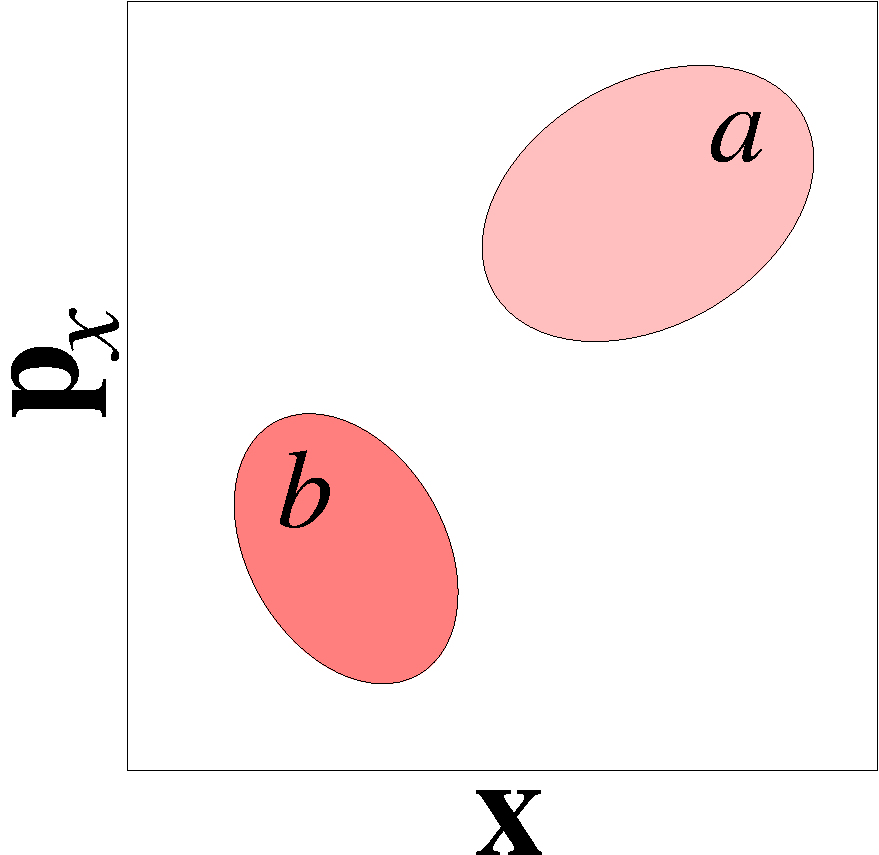
\includegraphics[width=4cm]{figures/overlap1}
          {\bfseries \sffamily (a)}
          \hfill
          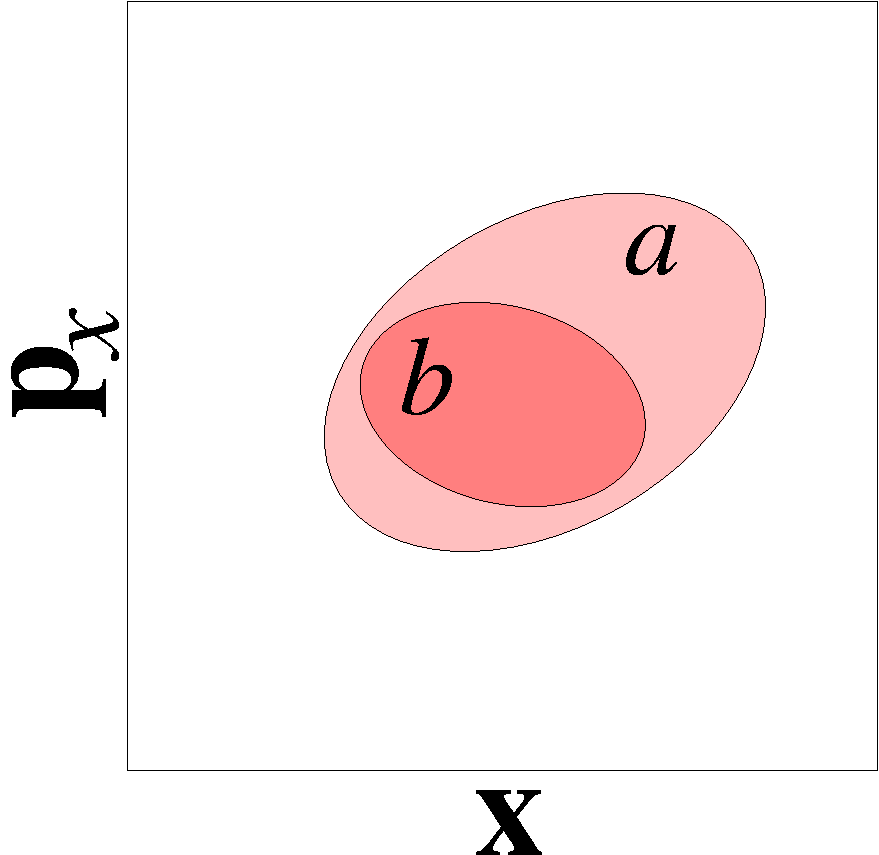
\includegraphics[width=4cm]{figures/overlap2}
          {\bfseries \sffamily (b)}
          \hfill
          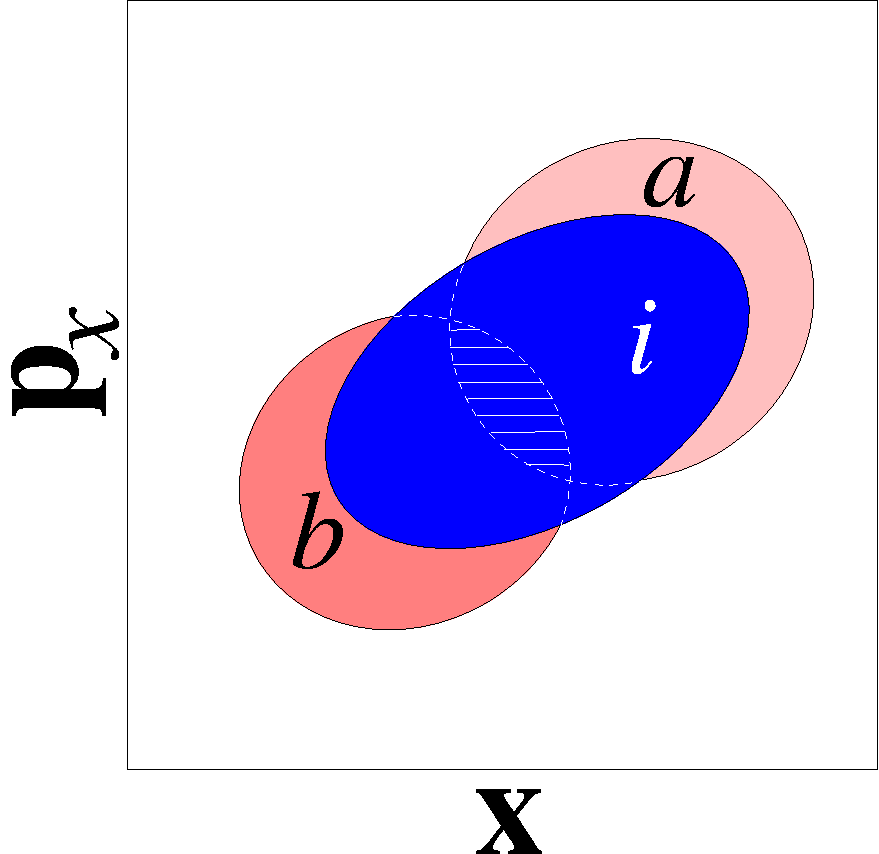
\includegraphics[width=4cm]{figures/overlap3}
          {\bfseries \sffamily (c)}}
  \caption{Convergence of an FEP calculation. If the ensembles representative
           of states $a$ and $b$ are too disparate, equation~({\ref{fep}}) will
           not converge {\bfseries \sffamily (a)}.
           If, in sharp contrast, the configurations of
           state $b$ form a subset of the ensemble of configurations
           characteristic of state $a$, the simulation is expected
           to converge {\bfseries \sffamily (b)}.
           The difficulties reflected in case {\bfseries \sffamily (a)} may be
           alleviated by the introduction of mutually overlapping intermediate
           states that connect $a$ to $b$ {\bfseries \sffamily (c)}. It should be
           mentioned that in practice, the kinetic contribution, ${\cal T}({\bf p}_x)$,
           is assumed to be identical for state $a$ and state $b$.
           \label{fig:overlap}}
\end{figure}


Convergence of equation~({\ref{fep}}) implies that low--energy configurations
of the target state, $b$, are also configurations of the reference state, $a$,
thus resulting in an appropriate overlap of the corresponding ensembles --- see
Figure~\ref{fig:overlap}. In practice, transformation between the two
thermodynamic states is replaced by a series of transformations between
non--physical, intermediate states along a well--delineated pathway that
connects $a$ to $b$. This pathway is characterized by the general extent
parameter ~\cite{Beveridge1989,Mark1998,King1993,Kirkwood1935}, $\lambda$, that
makes the Hamiltonian and, hence, the free energy, a continuous function of
this parameter between $a$ and $b$:


\begin{equation}
\Delta A_{a \rightarrow b} = -\frac{1}{\beta} \ \sum_{i = 1}^N \ln
                              \left\langle \exp\left\{-\beta
                                               \left[{\cal H}({\bf x}, {\bf p}_x; \lambda_{i+1}) -
                                                     {\cal H}({\bf x}, {\bf p}_x; \lambda_i)
                                               \right]
                                               \right\}
                                               \right\rangle_i
\label{windows}
\end{equation}


Here, $N$ stands for the number of intermediate stages, or ``windows''
between the initial and the final states --- see Figure~\ref{fig:overlap}.



\subsubsection{Thermodynamic Integration }

An alternative to the perturbation formula for free energy calculation is
Thermodynamic Integration (TI). With the TI method, the free energy is given
as~\cite{Kirkwood1935,mccammon_91_1,frenkel_2002}:


\begin{equation}
\Delta A =  \int_0^1 \left<\frac{\partial
{\cal H}({\bf x}, {\bf p}_x; \lambda)}{\partial \lambda}\right>_\lambda d\lambda
\end{equation}


In the multi-configuration thermodynamic integration approach
~\cite{mccammon_91_1} implemented in NAMD, $ \left<\partial {\cal H}({\bf x},
{\bf p}_x; \lambda) / \partial \lambda~\right>_\lambda $, the ensemble average
of the derivative of the internal energy with respect to $\lambda$, is
collected for a series of discrete $\lambda$ values and written to {\tt
alchOutFile}. These values are analyzed by the separately distributed script
{\tt NAMD\_ti.pl}, which performs the integration of individual energy
components and reports back the total $\Delta A$ values for the transformation.



\subsection{Implementation of the free energy methods in NAMD}
\label{section:fepparameters}


The procedures implemented in NAMD are particularly
adapted for performing free
energy calculations that split the $\lambda$
reaction path into a number of non--physical,
intermediate states, or ``windows''. Separate simulations
can be started for each window.
Alternatively, the {\sc Tcl} scripting ability of
NAMD can be employed advantageously
to perform the complete simulation in a single run.
An example, making use of such a script, is supplied at the end
of this section.

The following keywords can be used to run alchemical free
energy calculations.  The attention of the user is directed to a novel
hierarchy of parameters controlling both FEP and TI implementations.
Back-compatibility with configuration files running on previous versions of
NAMD is nevertheless ensured by means of aliased commands.

\begin{itemize}
\item
\NAMDCONFWDEF{alchOn}{ Is an alchemical transformation to be performed? } {{\tt
on} or {\tt off}} {{\tt off}} {Turns on alchemical transformation methods in
NAMD.}

\item
\NAMDCONFWDEF{alchMethod}{ Which method is to be employed for the alchemical
transformation? } {{\tt fep} or {\tt ti}} {{\tt ti} if only {\tt alchLambda} is
specified; {\tt fep} if {\tt alchLambdaPlusDelta} / {\tt alchLambdaMinusDelta}
are specified} {Turns on Hamiltonian scaling and ensemble averaging for
alchemical FEP or TI.}


\item
\NAMDCONF{alchLambda}{ Current value of the coupling parameter } {positive
decimal between 0.0 and 1.0} {The coupling parameter value determining the
progress of the perturbation for FEP or TI.}

\item
\NAMDCONF{alchLambdaPlusDelta}{Forward projected value of the coupling
parameter} {positive decimal between 0.0 and 1.0} {The {\tt
alchLambdaPlusDelta} value corresponds to the coupling parameter to be used for
sampling in the next window.  The free energy difference between {\tt
alchLambdaPlusDelta} and {\tt alchLambda} is calculated.  Through simulations
at progressive values of {\tt alchLambda} and {\tt alchLambdaPlusDelta} the
total free energy difference may be determined.}

\item
\NAMDCONF{alchLambdaMinusDelta}{Backward projected value of the coupling parameter}
{positive decimal between 0.0 and 1.0}
{The {\tt alchLambdaMinusDelta} value corresponds to the coupling parameter to be
used for sampling in the previous window, assuming that a double-wide sampling
simulation is being performed, whereby both the forward and the backward
transformations are computed explicitly.  The free energy difference
between {\tt alchLambdaMinusDelta} and {\tt alchLambda} is calculated.  Through
simulations at progressive values of {\tt alchLambda} and {\tt alchLambdaMinusDelta}
the total free energy difference may be determined.}

\item
\NAMDCONFWDEF{alchEquilSteps}{Number of equilibration steps in a window,
prior to data collection}
{positive integer less than {\tt numSteps} or {\tt run}}
{0}
{In each window {\tt alchEquilSteps} steps of equilibration can be
performed before ensemble averaging is initiated. The output also contains
the data gathered during equilibration and is meant for analysis of
convergence properties of the alchemical free energy calculation.}

\item
\NAMDCONFWDEF{alchFile}{{\tt pdb} file with perturbation flags}
{filename}
{coordinates}
{{\tt pdb} file to be used for indicating the status of all
atoms pertaining to the system, with respect to the alchemical transformation.
If this parameter is not declared specifically, then the
{\tt pdb} file specified by
{\tt coordinates} is utilized for this information.}

\item
\NAMDCONFWDEF{alchCol}{Column in the {\tt alchFile} that carries
                      the perturbation flag}
{X, Y, Z, O or B}
{B}
{Column of the {\tt pdb} file to use for retrieving the status
of each atom, \ie a flag that indicates which atom will be perturbed
in the course of the alchemical transformation.
A value of {\tt -1} in the specified column indicates that the atom will
vanish as $\lambda$ moves from 0 to 1, whereas a value of {\tt 1}
indicates that it will grow.}

\item
\NAMDCONFWDEF{alchOutFreq}{Frequency of free energy output in time--steps}
{positive integer}
{5}
{Every {\tt alchOutFreq} number of MD steps, the output file
{\tt alchOutFile} is updated by dumping energies that are
used for ensemble averaging.
This variable could be set to {\tt 1} to include all the
configurations for ensemble averaging. Yet, it is recommended
to update {\tt alchOutFile}  energies at longer intervals
to avoid large files containing highly correlated data, unless a post--treatment,
\eg Bennett's acceptance ratio (BAR)~\cite{Bennett1976} or simple overlap
sampling (SOS)~\cite{Lu2004}, is to be performed.}

\item
\NAMDCONFWDEF{alchOutFile}{Alchemical free energy output filename}
{filename}
{{\tt outfilename}}
{An output file named {\tt alchOutFile},
containing the FEP energies or TI derivatives, dumped every {\tt alchOutFreq} steps.}

\item
\NAMDCONFWDEF {alchVdWShiftCoeff}{Soft-core van der Waals radius-shifting coefficient}
{positive decimal}
{0} %CBH -- reconcile with SimParameters.C/.h
{This is a radius-shifting coefficient of $\lambda$ that is used
to construct the modified vdW interactions during alchemical free energy calculations.
Providing a positive value for {\tt alchVdWShiftCoeff} ensures that the vdW potential
is finite everywhere for small values of $\lambda$, which significantly improves the
accuracy and convergence of FEP and TI calculations, and also prevents overlapping particles
from making the simulation unstable. During FEP and TI, assuming $\lambda = 0$
denotes an absence of interaction, the interatomic distances used in
the Lennard-Jones potential are shifted according to ~\cite{zacharias_94_1}:
$r^2 \rightarrow r^2 + {\tt alchVdWShiftCoeff} \times (1 - \lambda)$
}

\item
\NAMDCONFWDEF {alchElecLambdaStart}{Value of $\lambda$ to introduce electrostatic interactions}
{positive decimal}
{0} %CBH -- reconcile with SimParameters.C/.h
{In order to avoid the so--called ``end-point catastrophes'', it is crucial to
avoid situations where growing particles overlap with existing particles with
an unbounded interaction potential, which would approach infinity as the
interaction distance approaches zero~\cite{BEUT1994}. One possible route for
avoiding overlap of unbounded electrostatic potentials consists of allowing a
bounded (soft-core) vdW potential, using a positive value of {\tt
alchVdWShiftCoeff}, to repel first all overlapping particles at low values of
$\lambda$. As $\lambda$ increases, once the particles are repelled, it becomes
safe to turn on FEP or TI electrostatics. {\tt alchElecLambdaStart} is the
value of the $\lambda$ at which electrostatic interactions are turned on and
linearly increased towards their nominal value. Below {\tt
alchElecLambdaStart}, electrostatic interactions are turned off for all
incoming and outgoing particles.}

\item
  \NAMDCONFWDEF {alchVdwLambdaEnd}{Value of $\lambda$ to cancel van der Waals interactions}
{positive decimal}
{1.0} %CBH -- reconcile with SimParameters.C/.h
{If the above {\tt alchElecLambdaStart} option is being used, it may be further
desirable to separate the scaling of van der Waals and electrostatic
interactions. {\tt alchVdwLambdaEnd} sets the value of $\lambda$ above which
all vdW interactions are fully enabled.}

\item
  \NAMDCONFWDEF {alchDecouple}{Disable scaling of nonbonded interactions within alchemical partitions}
{{\tt on} or {\tt off}} {{\tt off}} {With {\tt alchDecouple} set to {\tt on},
only nonbonded interactions of perturbed, incoming and outgoing atoms with
their environment are scaled, while interactions within the subset of perturbed
atoms are preserved. On the contrary, if {\tt alchDecouple} is set to {\tt
off}, interactions within the perturbed subset of atoms are also scaled and
contribute to the cumulative free energy. In most calculations, intramolecular
annihilation free energies are not particularly informative, and decoupling
ought to be preferred. Under certain circumstances, it may, however, be
desirable to scale intramolecular interactions, provided that the latter are
appropriately accounted for in the thermodynamic cycle~\cite{Chipot2007}. }

\item
  \NAMDCONFWDEF {alchDoubleWideSampling}{Will an FEP alchemical transformation be performed in the forward and the backward directions
  concomitantly?}
{{\tt on} or {\tt off}}
{{\tt off}} %CBH -- reconcile with SimParameters.C/.h
{Simultaneous alchemical transformations in the forward and the backward
 directions
 constitute a straightforward route towards the estimation of the error
 associated to the corresponding free energy calculations through their
 hysteresis. When set to {\tt on}, this option will request the
 concomitant evaluation of the ensemble averages over configurations
 representative of state $\lambda$, going (i) from $\lambda$ to $\lambda + \delta \lambda$
 (controlled by keyword {\tt alchLambdaPlusDelta}), and  (ii) from $\lambda$ to $\lambda - \delta \lambda$
 (controlled by keyword {\tt alchLambdaMinusDelta}). Accessing from a single free energy calculation
 the statistical information of both transformations is particularly useful for data post--processing, \eg
 BAR~\cite{Bennett1976} and SOS~\cite{Lu2004}, which have proven to improve the accuracy of the free--energy
 estimates over brute--force application of the FEP formula. It should be emphasized, however, that
 forward and backward transformations do not necessarily share the same convergence properties, so that,
 over finite--length simulations, free--energy differences will not be strictly equal.  }
\end{itemize}



\subsection{Examples of input files for running alchemical free energy calculations}


The first example illustrates the use of {\sc Tcl} scripting for running
an alchemical transformation with the FEP feature of NAMD. In this
calculation, $\lambda$ is changed continuously from 0 to 1
by increments of $\delta \lambda$ = 0.1.


\begin{tabular}{ll}
\begin{minipage}{8cm}
\begin{verbatim}
alch            on
alchMethod      fep
alchFile        ion.fep
alchCol         X
alchOutfile     ion.fepout
alchOutFreq     5
alchEquilSteps  5000

set Lambda0     0.0
set dLambda 0.1

while {$Lambda0 <= 1.0} {
 alchLambda $Lambda0
 set Lambda0 [expr \$Lambda0 + \$dLambda]
 alchLambdaPlusDelta $Lambda0
 run  10000
}
\end{verbatim}
\end{minipage}
&
\begin{minipage}{7.8cm}
%\newline
Turn FEP functionality on.
\newline
Alchemical Method to use.
\newline
File containing the information about growing/shrinking atoms
described in column {\tt X}.
\newline
Output file containing the free energy.
\newline
Frequency at which {\tt alchOutFreq} is updated.
\newline
Number of equilibration steps per $\lambda$--state.
\\[0.6cm]
Starting value of $\lambda$.
\newline
Increment of $\lambda$, \ie $\delta \lambda$.
\\[0.6cm]
{\sc Tcl} script to increment $\lambda$:
\newline
\hspace{0.4cm} (1) set {\tt alchLambda} value;
\newline
\hspace{0.4cm} (2) increment $\lambda$;
\newline
\hspace{0.4cm} (3) set {\tt alchLambdaPlusDelta} value;
\newline
\hspace{0.4cm} (4) run 10,000 MD steps.
\\
\end{minipage}
\end{tabular}


The user should be reminded that by setting {\tt run  10000},
10,000 MD steps will be performed, which includes the
preliminary {\tt alchEquilSteps} equilibration steps.
This means that here, the ensemble average of equation~({\ref{windows}})
will be computed  over 5,000 MD steps.


Alternatively, $\lambda$--states may be declared
explicitly, avoiding the use of {\sc Tcl} scripting:

\begin{tabular}{ll}
\begin{minipage}{8cm}
\begin{verbatim}
lambda          0.0
alchLambdaPlusDelta         0.1
run             10000
\end{verbatim}
\end{minipage}
&
\begin{minipage}{7.8cm}
(1) set {\tt alchLambda} value;
\newline
(2) set {\tt alchLambdaPlusDelta} value;
\newline
(3) run 10,000 MD steps.
\end{minipage}
\end{tabular}


This option is generally preferred to set up windows of diminishing
widths as $\lambda \rightarrow$ 0 or 1 --- a way to circumvent
end--point singularities caused by appearing atoms that may
clash with their surroundings.


The following second input is proposed for the measuring via TI the free energy
of a particle insertion.

\begin{verbatim}
    alch            on
    alchMethod      ti             # Enable thermodynamic integration
    alchFile        ion.alch.pdb   # PDB file with perturbation flags
    alchCol         B              # Perturbation flags in Beta column
    alchOutfile     ion.ti.out
    alchOutFreq     5
    alchEquilSteps  5000

    alchVdWShiftCoeff    1         # Enable soft-core vdW potential
    alchElecLambdaStart  0.1       # Introduce electrostatics for lambda > 0.1
    alchLambda 0
    run 10000
    alchLambda 0.00001
    run 10000
    alchLambda 0.0001
    run 10000
    alchLambda 0.001
    run 10000
    alchLambda 0.01
    run 10000

    set Lambda           0.1

    while {$Lambda <= 0.9} {
      alchLambda $Lambda
      run 10000
      set Lambda [expr $Lambda + 0.1]
    }

    alchLambda 0.99
    run 10000
    alchLambda 0.999
    run 10000
    alchLambda 0.9999
    run 10000
    alchLambda 0.99999
    run 10000
    alchLambda 1
    run 10000

\end{verbatim}

In this example, most input parameters are shared with FEP, except for the
specification of {\tt alchMethod ti} and the absence of {\tt
alchLambdaPlusDelta} or {\tt alchLambdaMinusDelta} parameters. Moreover, robust
sampling of the free energy of particle insertion is enabled by the use of
soft-core van der Waals scaling with the {\tt alchVdWShiftCoeff} parameter,
delayed introduction of electrostatics with a non-zero {\tt
alchElecLambdaStart} value, and very gradual scaling of $\lambda$ towards its
end points.



\subsection{Description of a free energy calculation output }


\subsubsection{Free Energy Perturbation }


When running FEP, the {\tt alchOutFile} contains electrostatic and van der Waals energy
data calculated for {\tt alchlambda} and {\tt lambda}, written every
{\tt alchOutFreq} steps. The column {\tt dE} is the energy
difference of the single configuration, {\tt dE\_avg} and {\tt dG}
are the instantaneous ensemble average of the energy and the calculated
free energy at the time step specified in column 2, respectively.
The temperature is specified in the penultimate column. Upon completion
of {\tt alchEquilSteps} steps, the calculation of {\tt dE\_avg} and
{\tt dG} is restarted. The accumulated net free energy change is written
at each lambda value and at the end of the simulation.
%FB this will confuse people and doesn't apply with non-linear vdW scaling
%The cumulative average energy {\tt dE\_avg} value may be summed using the
%trapezoidal rule to obtain an approximate TI
%estimate for the free energy change during the run. =====> WHERE WILL IT CONFUSE PEOPLE?


Whereas the FEP module of NAMD supplies free energy differences determined from
equation~({\ref{fep}}), the wealth of information available in {\tt
alchOutFile} may be utilized profitably to explore different routes towards the
estimation of $\Delta A$. Both BAR and SOS methods, which combine
advantageously \emph{direct} and \emph{reverse} transformations to improve
convergence and accuracy of the calculation, represent relevant alternatives to
brute--force application of the FEP formula~\cite{lu2004}.


Within the SOS framework, the free energy difference between states $\lambda_i$ and
$\lambda_{i+1}$ is expressed as:


\begin{equation}
\exp(-\beta \Delta A_{i \rightarrow i+1})  =
\frac{\displaystyle
      \left\langle \exp\left\{-\frac{\beta}{2}
                       \left[
                       {\cal H}({\bf x}, {\bf p}_x; \lambda_{i+1}) - {\cal H}({\bf x}, {\bf p}_x; \lambda_i)
                       \right]
                       \right\}
      \right\rangle_i}
      {\displaystyle
       \left\langle \exp\left\{-\frac{\beta}{2}
                       \left[
                       {\cal H}({\bf x}, {\bf p}_x; \lambda_i) - {\cal H}({\bf x}, {\bf p}_x; \lambda_{i+1})
                       \right]
                       \right\}
      \right\rangle_{i+1}}
\label{sos}
\end{equation}

\noindent and can be readily used with the statistical information provided by the forward and the backward runs.


\subsubsection{Thermodynamic Integration }


When running TI free energy calculations, the {\tt elec\_dU/dl} and {\tt
vdW\_dU/dl} values reported in {\tt alchOutFile} are the derivatives of the
internal energy with respect to $\lambda$ --- \ie $\frac{\partial
U}{\partial\lambda}$ for electrostatics and, van der Waals, respectively. {\tt
dU/dl} values are averages over the last {\tt alchOutFreq} steps. Cumulative
averages for each component are reported alongside in the {\tt \_avg} columns.


The electrostatics and vdW are separated following a partition scheme --- that
is, the ``appearing'' and the ``disappearing'' atoms are accounted for
separately. ``Partition 1'' contains those atoms whose interactions are
switched up as $\lambda$ increases --- \ie flagged with {\tt 1} in the {\tt
alchFile}. ``Partition 2'' represents those atoms whose interactions are
switched down as $\lambda$ increases --- \ie flagged with {\tt -1}. $\Delta A$
values for each component are obtained by integrating from $\lambda=0$ to $1$
using the respective {\tt ELEC / VDW LAMBDA} listed for each partition after
the title.


Analysis is handled by the {\tt NAMD\_ti} script, available from
\begin{quote}
http://www.ks.uiuc.edu/Research/namd/utilities/
\end{quote}


Although the output format of {\tt NAMD\_ti.pl } may appear to lend itself easily to interpretation of the
individual contributions to the free energy total (elec and vdW for each partition), this is rarely
appropriate as these values are path-dependent. For example, an output such as


\begin{verbatim}
          |-----------------------------------------------|
          |         |    elec   |    vdW    |   Subtotal  |
          |-----------------------------------------------|
          | Part. 1 |   -0.5748 |   -6.3452 |    -6.9200  |
          | Part. 2 |    0.5391 |    4.9387 |     5.4778  |
          |-----------------------------------------------|
          | Subtotal|    0.6048 |    0.3293 |   -12.3978  |
          |-----------------------------------------------|
          Total deltaG for transition lambda 0 -> 1: -12.3978
\end{verbatim}


\noindent may encourage interpretations along the lines of "the free energy for
switching on the van der Waals interactions for the atoms of partition 1 was
-6.35kcal/mol". This is only correct in the very narrow context of the
simulation setup and parameters used in this case and is not informative in a
broader sense.


\begin{figure}[ht]
  \center{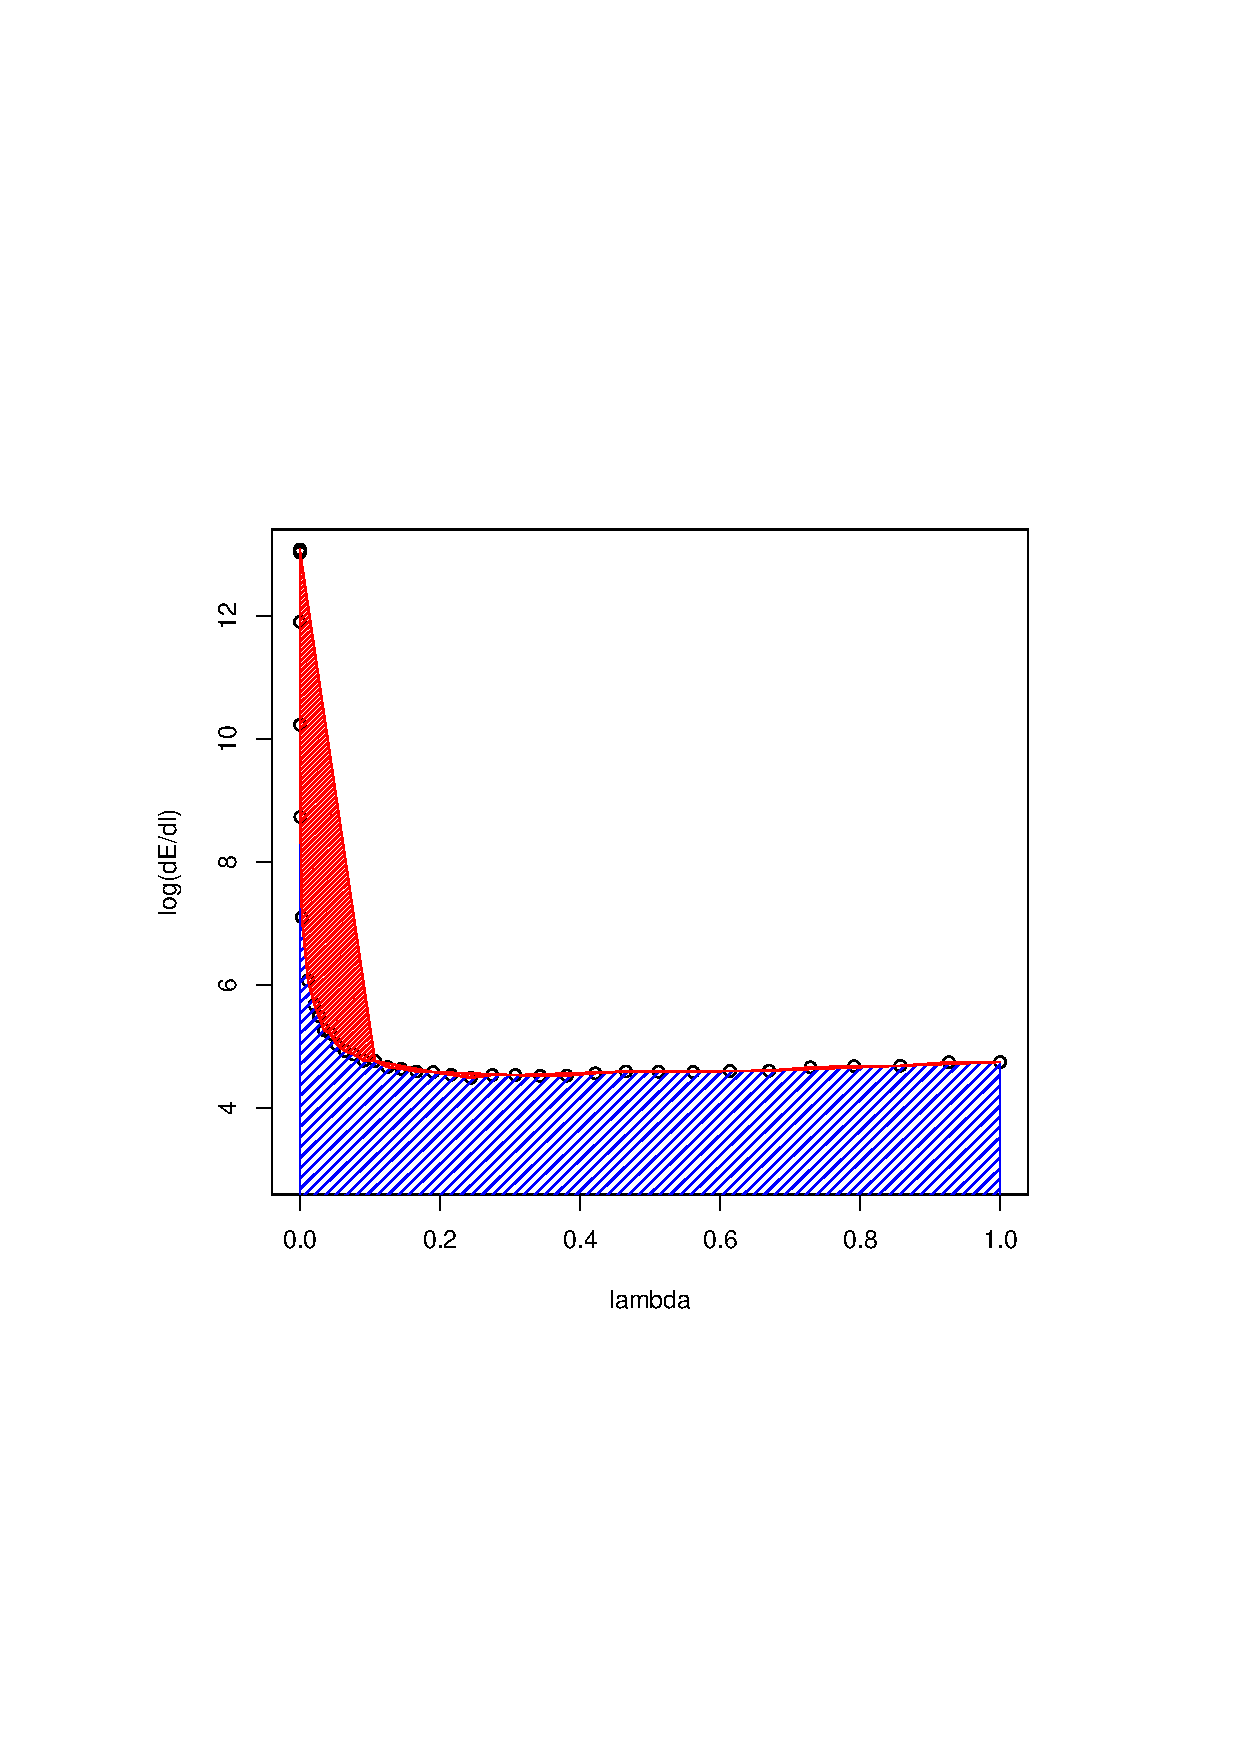
\includegraphics[width=7cm]{figures/TI}}
  \caption{Sample TI data ($log(\left<\frac{\partial U}{\partial\lambda}\right>)$ against $\lambda$). The blue shaded
  area shows the integral with fine sampling close to the end point. The red area
  shows the difference when $\lambda$ values are more sparse. In this example,
  insufficient sampling before $\lambda$ $\simeq$0.1 can result in a large overestimation
  of the integral. Beyond $\simeq$0.2, sparser sampling is justified as dE/d$\lambda$ is not
  changing quickly.}
  \label{fig:TI}
\end{figure}


The choice of $\lambda$ values will depend on the application, but in general
it is important to examine the shape of the curve to ensure that sampling is
adequate to give a good estimate of the integral. In particular, it will be
necessary to sample more finely towards the end points in order to accurately
account for the strong repulsive van der Waals forces encountered when
inserting particles into a system (see Figure~\ref{fig:TI}).



%\bibliographystyle{unsrt}
%\bibliography{../../LaTeX/Bibliography/data_base}

%\end{document}
